%%%%%%%%%%%%%%%%%%%%%%%%%%%%%%%%%%%%%
%                                   %
% Compile with XeLaTeX and biber    %
%                                   %
% Questions or comments:            %
%                                   %
% joshua dot mcneill at uga dot edu %
%                                   %
%%%%%%%%%%%%%%%%%%%%%%%%%%%%%%%%%%%%%

\documentclass{beamer}
  % Read in standard preamble (cosmetic stuff)
  %%%%%%%%%%%%%%%%%%%%%%%%%%%%%%%%%%%%%%%%%%%%%%%%%%%%%%%%%%%%%%%%
% This is a standard preamble used in for all slide documents. %
% It basically contains cosmetic settings.                     %
%                                                              %
% Joshua McNeill                                               %
% joshua dot mcneill at uga dot edu                            %
%%%%%%%%%%%%%%%%%%%%%%%%%%%%%%%%%%%%%%%%%%%%%%%%%%%%%%%%%%%%%%%%

% Beamer settings
% \usetheme{Berkeley}
\usetheme{CambridgeUS}
% \usecolortheme{dove}
% \usecolortheme{rose}
\usecolortheme{seagull}
\usefonttheme{professionalfonts}
\usefonttheme{serif}
\setbeamertemplate{bibliography item}{}

% Packages and settings
\usepackage{fontspec}
  \setmainfont{Charis SIL}
\usepackage{hyperref}
  \hypersetup{colorlinks=true,
              allcolors=blue}
\usepackage{graphicx}
  \graphicspath{{../../figures/}}
\usepackage[normalem]{ulem}
\usepackage{enumerate}

% Document information
\author{M. McNeill}
\title[FREN2001]{Français 2001}
\institute{\url{joshua.mcneill@uga.edu}}
\date{}

%% Custom commands
% Lexical items
\newcommand{\lexi}[1]{\textit{#1}}
% Gloss
\newcommand{\gloss}[1]{`#1'}
\newcommand{\tinygloss}[1]{{\tiny`#1'}}
% Orthographic representations
\newcommand{\orth}[1]{$\langle$#1$\rangle$}
% Utterances (pragmatics)
\newcommand{\uttr}[1]{`#1'}
% Sentences (pragmatics)
\newcommand{\sent}[1]{\textit{#1}}
% Base dir for definitions
\newcommand{\defs}{../definitions}


  % Packages and settings
  \usepackage{tikz}
  \usepackage{adjustbox}
  \usepackage[backend=biber, style=apa]{biblatex}
    \addbibresource{../references/References.bib}

  % Document information
  \subtitle[Acoustic Phonetics]{Acoustic Phonetics}

  %% Custom commands
  % Subsection/frame titles
  \newcommand{\suboneone}{Definition}
  \newcommand{\subtwoone}{Simple sound waves}
  \newcommand{\subtwotwo}{Complex sound waves}
  \newcommand{\subtwothree}{Vowels}
  \newcommand{\subtwofour}{Consonants}
  \newcommand{\subtwofive}{Resources and practice}

\begin{document}
  % Read in the standard intro slides (title page and table of contents)
  %%%%%%%%%%%%%%%%%%%%%%%%%%%%%%%%%%%%%%%%%%%%%%%%%%%%%%%%%%%%%%%%
% This is a standard set of intro slides used in for all slide %
% documents. It basically contains the title page and table of %
% contents.                                                    %
%                                                              %
% Joshua McNeill                                               %
% joshua dot mcneill at uga dot edu                            %
%%%%%%%%%%%%%%%%%%%%%%%%%%%%%%%%%%%%%%%%%%%%%%%%%%%%%%%%%%%%%%%%

\begin{frame}
  \titlepage
  \tiny{Office: % Basically a variable for office hours location
Gilbert 121\\
        Office hours: % Basically a variable for office hours
 lundi, mercredi, vendredi 10:10--11:10
}
\end{frame}

\begin{frame}
  \tableofcontents[hideallsubsections]
\end{frame}

\AtBeginSection[]{
  \begin{frame}
    \tableofcontents[currentsection,
                     hideallsubsections]
  \end{frame}
}


  \section{What is acoustic phonetics?}
    \subsection{\suboneone}
      \begin{frame}{\suboneone}
        \only<1-3>{
          \begin{block}{}
            The three broad areas of phonetics:
            \begin{itemize}
              \item Articulatory phonetics
              \item \alert<2->{Acoustic phonetics}
              \item Auditory phonetics
            \end{itemize}
          \end{block}
          \begin{definition}<2-3>
            % Read in the definition of articulatory phonetics
            % Acoustic phonetics
The study of the acoustic properties of speech sounds and their transmission

          \end{definition}
          \begin{alertblock}<3>{}
            We're no longer looking at how sounds are produced but what they look like when measured
          \end{alertblock}
        }
        \only<4->{
          \begin{block}{Why looking instead of listening?}
            \uncover<5->{
              Because listeners' impressions of sounds can differ
              \begin{itemize}
                \item Instead we use technology, mainly Praat
                \item \url{http://www.fon.hum.uva.nl/praat/}
              \end{itemize}
            }
          \end{block}
          \begin{block}<6->{Two types of visualizations}
            \begin{itemize}
              \item Waveform
              \item Spectrogram
            \end{itemize}
          \end{block}
        }
      \end{frame}

  \section{All about sound}
    \subsection{\subtwoone}
      \begin{frame}[t]{\subtwoone}
        \only<1-2>{
          \begin{alertblock}{A sound wave}
            % Sound wave
An oscillation of pressure in the air

          \end{alertblock}
        }
        \only<2>{
          \begin{columns}
            \column{0.5\textwidth}
              \begin{minipage}[c][0.6\textheight]{\linewidth}
                \begin{block}{The simple kind}
                  There is some consistent, steady pattern to the \href{https://youtu.be/PyD9cMarVJk}{sound wave}
                \end{block}
              \end{minipage}
            \column{0.5\textwidth}
              % Simple water ripple
              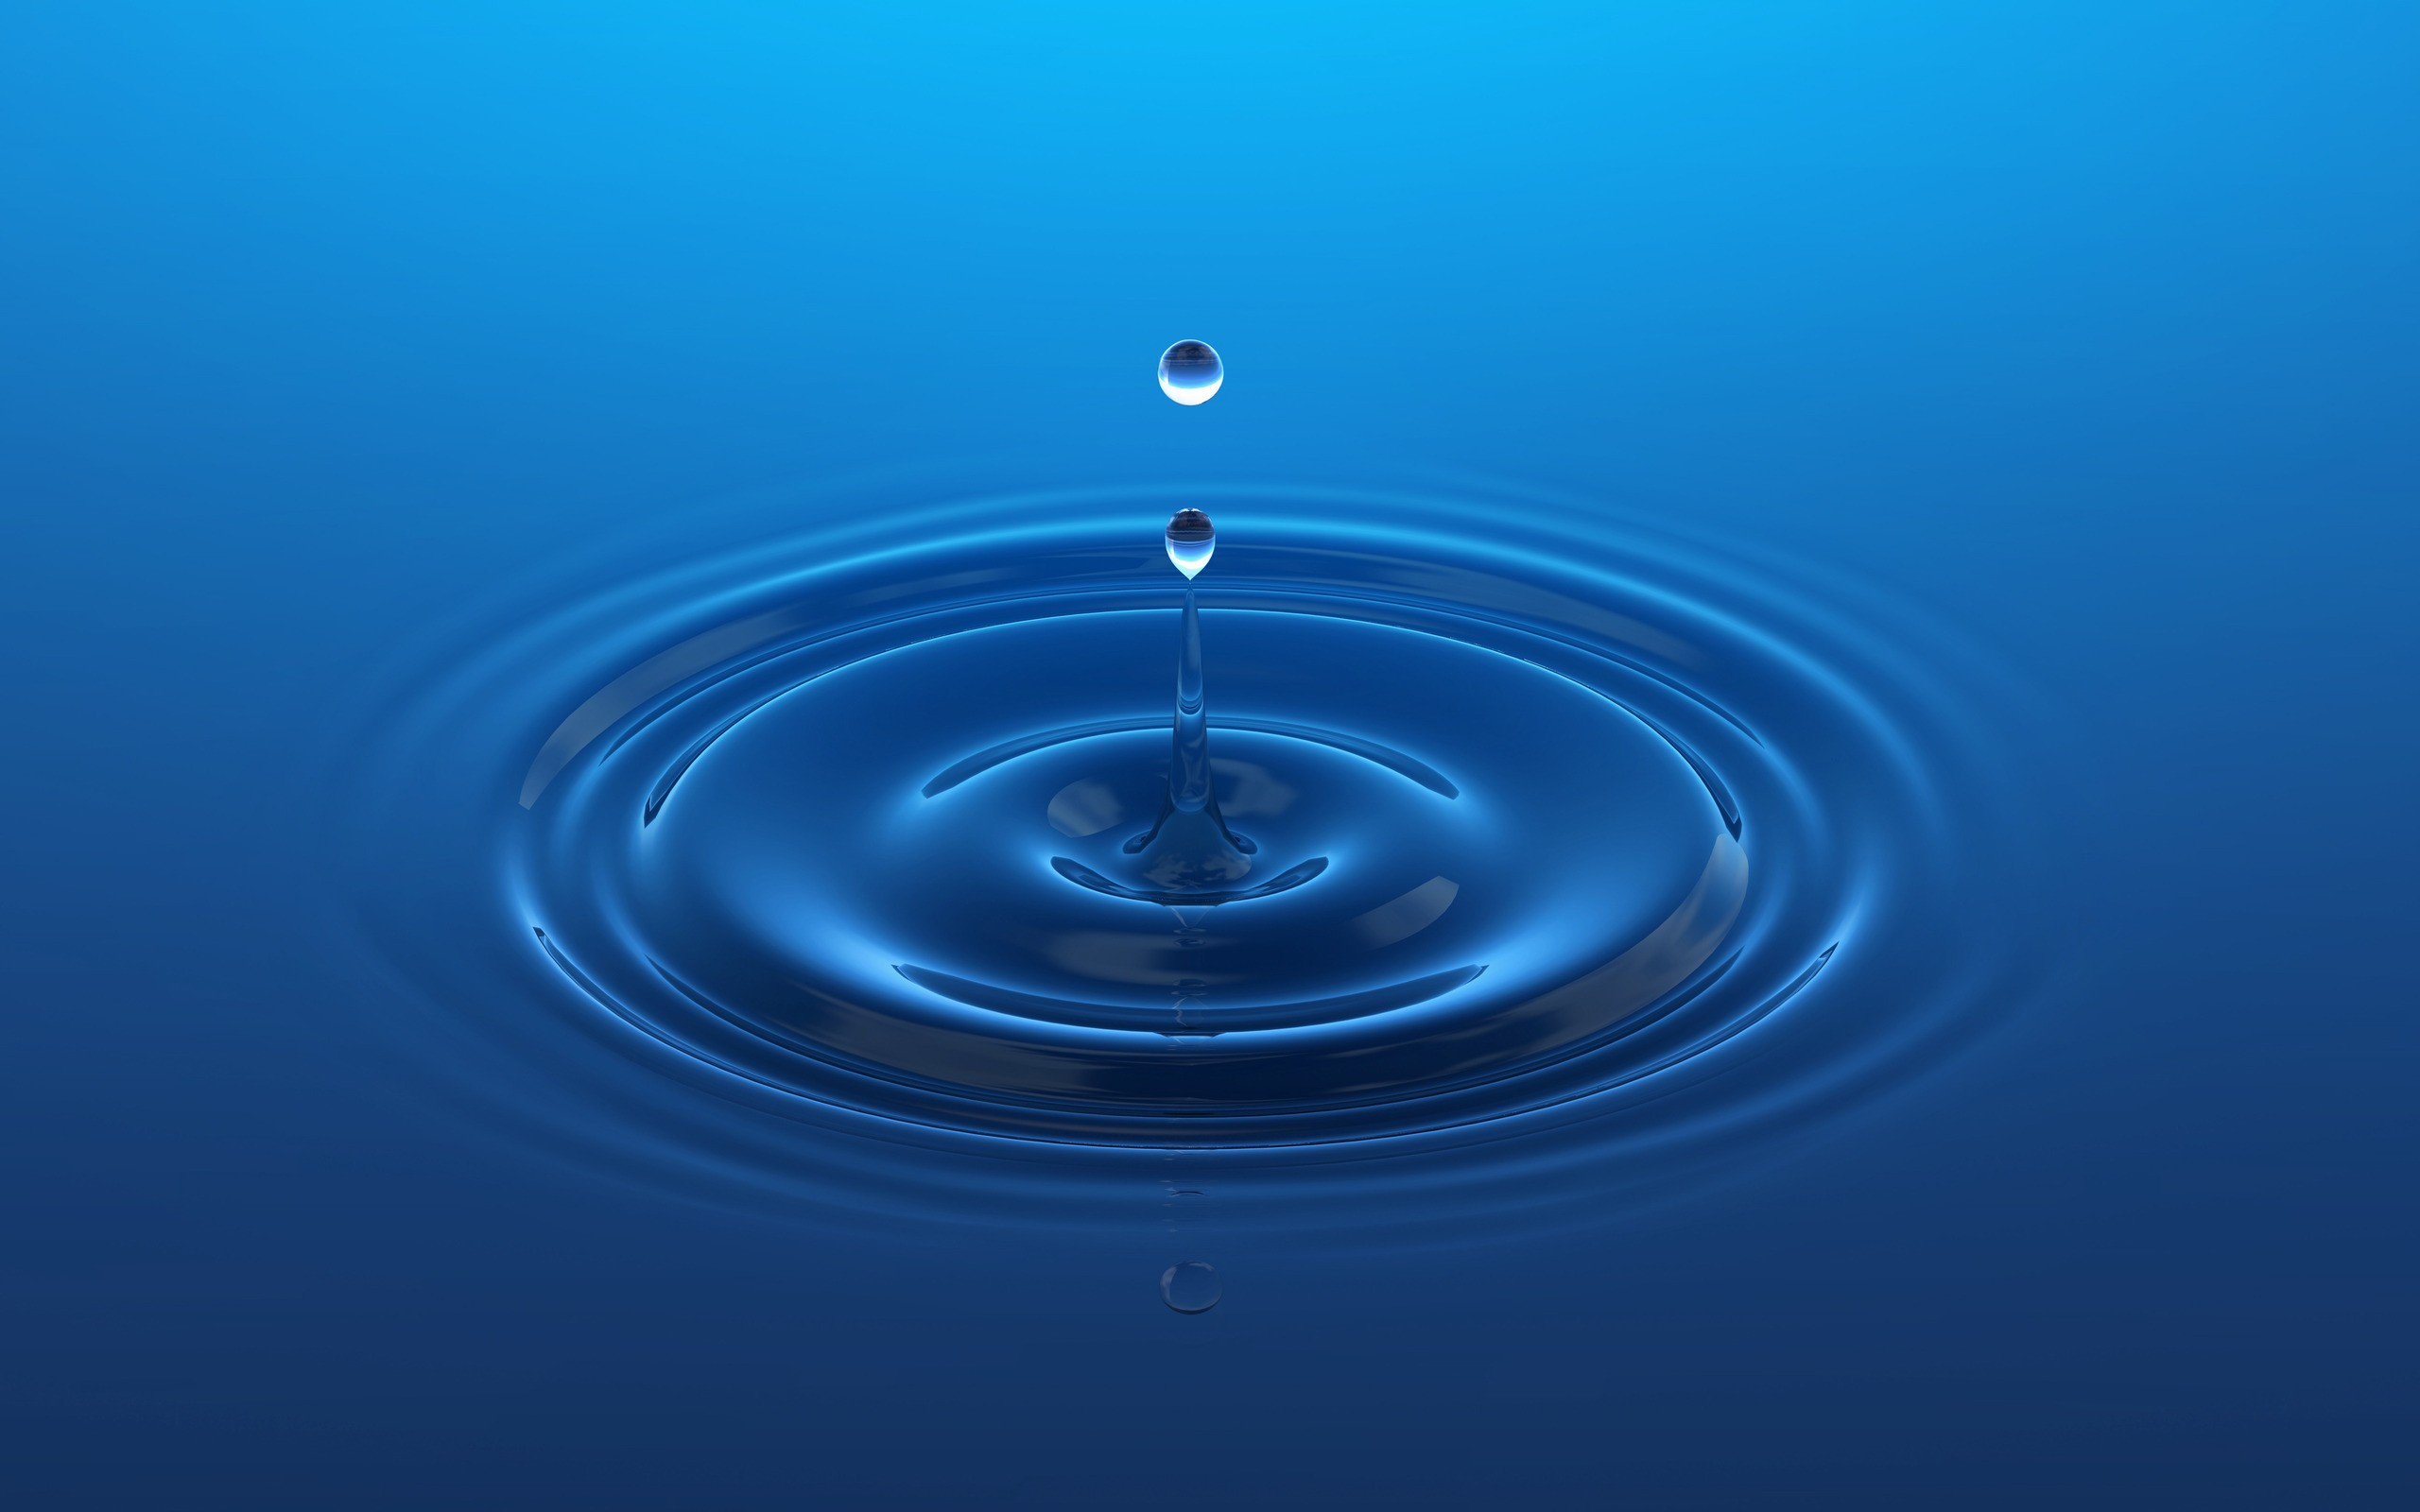
\includegraphics[scale=0.055]{ripple_simple.jpg}
          \end{columns}
        }
        \only<3-6>{
          \begin{columns}
            \column{0.5\textwidth}
              \only<3>{
                \begin{alertblock}{A waveform}
                  % Definition of waveform
                  % Waveform
A visualization for sound waves with time on the x-axis and amplitude on the y-axis

                \end{alertblock}
              }
              \only<4-6>{
                \begin{block}{Two aspects of a sound wave}
                  \begin{itemize}
                    \item \alert{Frequency}: % Frequency
A measure of how many cycles per second (i.e., Hz) there are in a sound wave

                    \item \alert{Amplitude}: % Amplitude
A measure of how loud a sound is, typically measured in decibels (dB)

                  \end{itemize}
                \end{block}
              }
            \column{0.5\textwidth}
              \uncover<3-6>{
                % Basic waveform
                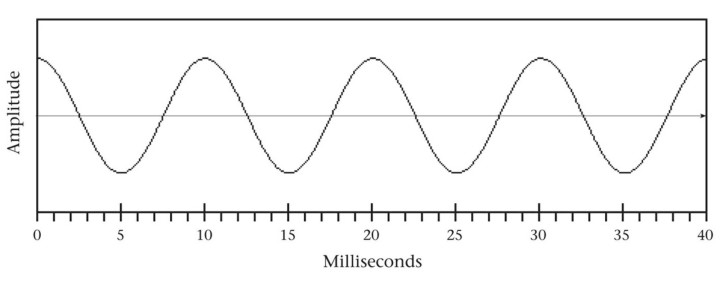
\includegraphics[scale=0.4]{waveform_basic.jpg}
              }
              \uncover<5-6>{
                % Higher frequency
                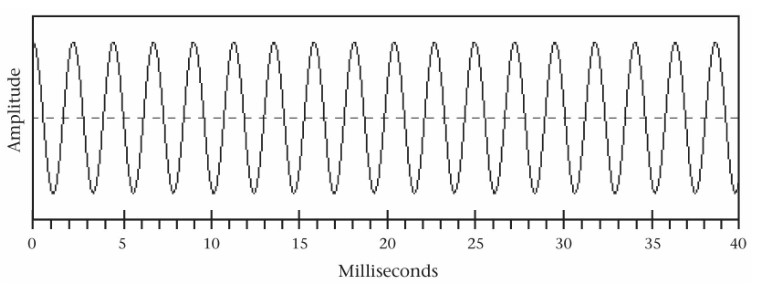
\includegraphics[scale=0.385]{waveform_high_freq.jpg}
              }
              \uncover<6>{
                % Lower amplitude
                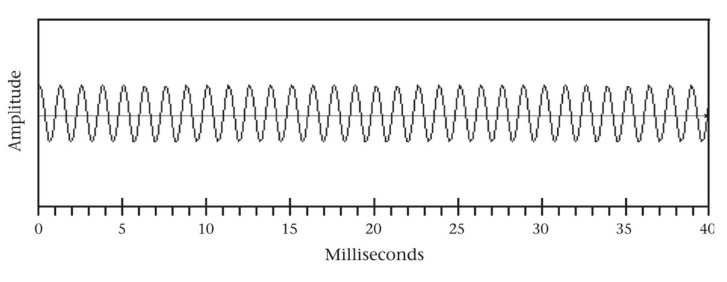
\includegraphics[scale=0.4]{waveform_low_amp.jpg}
              }
          \end{columns}
        }
      \end{frame} % Maybe give frequency range of human hearing and speech

    \subsection{\subtwotwo}
      \begin{frame}{\subtwotwo}
          \begin{columns}
            \column{0.48\textwidth}
              \begin{minipage}[c][0.6\textheight]{\linewidth}
                \only<1-3>{
                  \begin{block}{Battling it out}
                    Multiple simple sound waves overlapping and colliding
                  \end{block}
                }
                \only<4->{
                  \begin{block}{To make things more complicated}
                    The vocal tract acts as a filter on the resulting complex sound waves
                  \end{block}
                  \begin{alertblock}<5->{}
                    Waveforms ultimately only tell us about overall amplitude
                  \end{alertblock}
                }
              \end{minipage}
            \column{0.48\textwidth}
              \begin{minipage}[c][0.6\textheight]{\linewidth}
                \only<1>{
                % Complex water ripples
                \includegraphics[scale=0.04]{ripple_complex.jpg}
                }
                \only<2->{
                  % Basic waveform
                  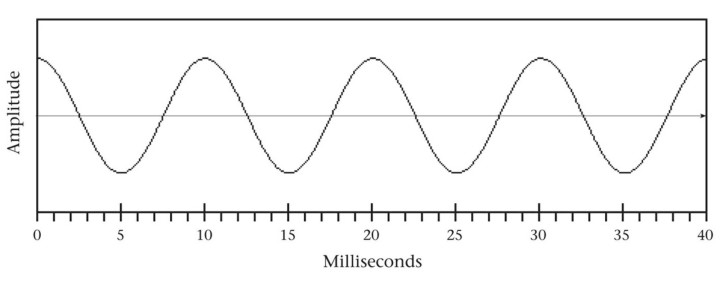
\includegraphics[scale=0.4]{waveform_basic.jpg}

                  % Lower amplitude
                  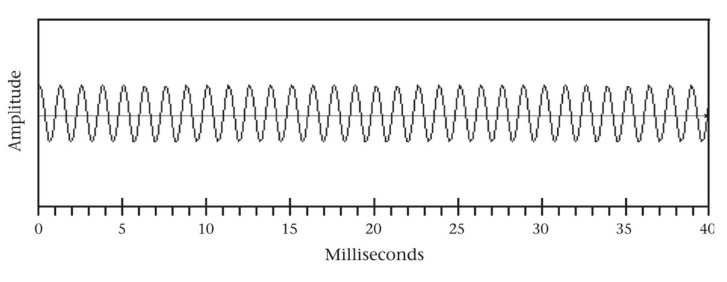
\includegraphics[scale=0.4]{waveform_low_amp.jpg}

                  \uncover<3->{
                    % Complex composite
                    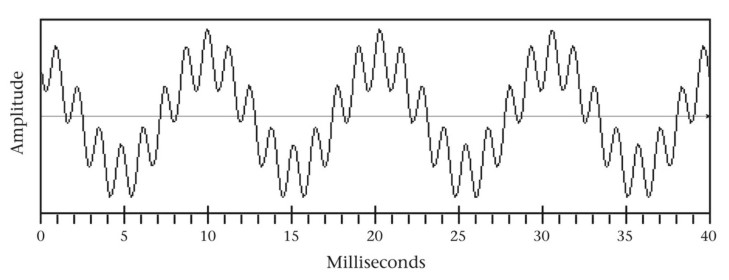
\includegraphics[scale=0.4]{waveform_complex.jpg}
                  }
                }
              \end{minipage}
          \end{columns}
      \end{frame}

    \subsection{\subtwothree}
      \begin{frame}{\subtwothree}
        \only<1>{
          \begin{block}{}
            Vowels can be described acoustically by measuring their formants
          \end{block}
          \begin{alertblock}{Formant}
            % Definition of a formant
            % Formant
A frequency whose amplitude is augmented relative to the surrounding frequencies when producing vowels

          \end{alertblock}
          \begin{block}{There are two important formants for vowels}
            \begin{itemize}
              \item \alert{Formant 1 (F1)}: % F1
The formant that represents vowel height

              \item \alert{Formant 2 (F2)}: % F2
The formant that represents vowel advancement

            \end{itemize}
          \end{block}
        }
        \only<2>{
          \begin{block}{}
            A plot of a speaker's vowel space (right) using formant frequencies looks a lot like a vowel chart (left)
          \end{block}
          \begin{columns}
            \column{0.45\textwidth}
              \begin{adjustbox}{width=4.5cm}
                %%%%%%%%%%%%%%%%%%%%%%%%%%%%%%%%%%%%%%%%%%%%%%%%%%%%%%%%%%%%%%%%%%%%%%%%%%%%%%%%%%%%%
% This creates an English IPA chart for vowels                                      %
%                                                                                   %
% Compiled from material_IPA_en_chart.tex when a                                    %
% standalone document is needed                                                     %
%                                                                                   %
% Code is only slightly modified from:                                              %
%   https://tex.stackexchange.com/questions/156955/tikz-pgf-linguistics-vowel-chart %
%                                                                                   %
% -Joshua McNeill (joshua dot mcneill at uga dot edu)                               %
%%%%%%%%%%%%%%%%%%%%%%%%%%%%%%%%%%%%%%%%%%%%%%%%%%%%%%%%%%%%%%%%%%%%%%%%%%%%%%%%%%%%%

% Custom command
\def\V(#1,#2){barycentric cs:hf={(3-#1)*(2-#2)},hb={(3-#1)*#2},lf={#1*(2-#2)},lb={#1*#2}}

% Chart
\begin{tikzpicture}[scale=3]
  \large
  \tikzset{
    vowel/.style={fill=white, anchor=mid, text depth=0ex, text height=1ex},
    dot/.style={circle,fill=black,minimum size=0.4ex,inner sep=0pt,outer sep=-1pt},
  }
  \coordinate (hf) at (0,2); % high front
  \coordinate (hb) at (2,2); % high back
  \coordinate (lf) at (1,0); % low front
  \coordinate (lb) at (2,0); % low back
  \def\V(#1,#2){barycentric cs:hf={(3-#1)*(2-#2)},hb={(3-#1)*#2},lf={#1*(2-#2)},lb={#1*#2}}

  % Draw the horizontal lines first.
  \draw (\V(0,0)) -- (\V(0,2));
  \draw (\V(1,0)) -- (\V(1,2));
  \draw (\V(2,0)) -- (\V(2,2));
  \draw (\V(3,0)) -- (\V(3,2));

  % Place all the unrounded-rounded pairs next, on top of the horizontal lines.
  \path (\V(0,0))     node[vowel, left] {i}          node[vowel, right] { }          node[dot] {};
  \path (\V(0,1))     node[vowel, left] { }          node[vowel, right] { }          node[dot] {};
  \path (\V(0,2))     node[vowel, left] { }          node[vowel, right] {u}          node[dot] {};
  \path (\V(0.5,0.4)) node[vowel, left] {\textbf{ɪ}} node[vowel, right] { }          node[   ] {};
  \path (\V(0.5,1.6)) node[vowel, left] { }          node[vowel, right] {\textbf{ʊ}} node[   ] {};
  \path (\V(1,0))     node[vowel, left] {e}          node[vowel, right] { }          node[dot] {};
  \path (\V(1,1))     node[vowel, left] { }          node[vowel, right] { }          node[dot] {};
  \path (\V(1,2))     node[vowel, left] { }          node[vowel, right] {o}          node[dot] {};
  \path (\V(2,0))     node[vowel, left] {\textbf{ɛ}} node[vowel, right] { }          node[dot] {};
  \path (\V(2,1))     node[vowel, left] { }          node[vowel, right] { }          node[dot] {};
  \path (\V(2,2))     node[vowel, left] {\textbf{ʌ}} node[vowel, right] {ɔ}          node[dot] {};
  \path (\V(2.5,0))   node[vowel, left] {\textbf{æ}} node[vowel, right] { }          node[   ] {};
  \path (\V(3,0))     node[vowel, left] {a}          node[vowel, right] { }          node[dot] {};
  \path (\V(3,2))     node[vowel, left] {ɑ}          node[vowel, right] { }          node[dot] {};

  % Draw the vertical lines.
  \draw (\V(0,0)) -- (\V(3,0));
  \draw (\V(0,1)) -- (\V(3,1));
  \draw (\V(0,2)) -- (\V(3,2));

  % Place the unpaired symbols last, on top of the vertical lines.
  \path (\V(1.5,1))   node[vowel]       {\textbf{ə}};
  \path (\V(-0.25,0)) node[vowel]       {front};
  \path (\V(-0.25,1)) node[vowel]       {central};
  \path (\V(-0.25,2)) node[vowel]       {back};
  \path (\V(0,-0.5))  node[vowel]       {high};
  \path (\V(1,-0.8))  node[vowel]       {high-mid};
  \path (\V(2,-1.55)) node[vowel]       {low-mid};
  \path (\V(3,-2.95)) node[vowel]       {low};
\end{tikzpicture}

              \end{adjustbox}
            \column{0.55\textwidth}
              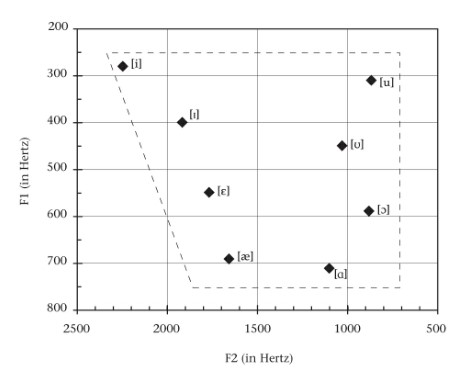
\includegraphics[scale=0.69]{vowel_space.jpg}
          \end{columns}
        }
        \only<3->{
          \begin{alertblock}{Spectrograms}
            % Definition of spectrogram
            % Spectrogram
A visualization for sound waves with time on the x-axis, frequency on the y-axis, and amplitude represented by shade

          \end{alertblock}
          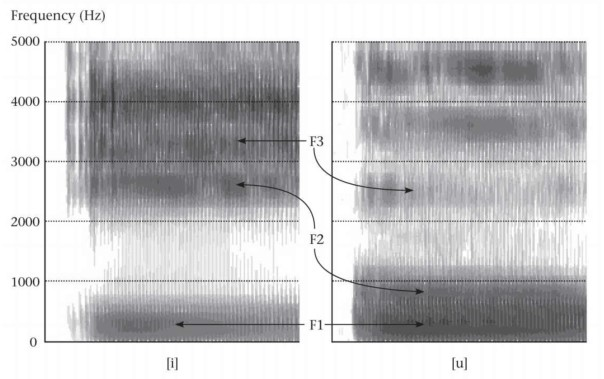
\includegraphics[scale=0.7]{spectrogram_formants.jpg}
        }
      \end{frame}

    \subsection{\subtwofour}
      \begin{frame}{\subtwofour}
        \only<1>{
          \begin{block}{Stops}
            Appear as gaps on a spectrogram
            \begin{itemize}
              \item Place of articulation can be determined by how the formants shift from a consonant to the following vowel
              \item Voiced sounds have a \alert{voice bar} at the bottom
            \end{itemize}
          \end{block}
          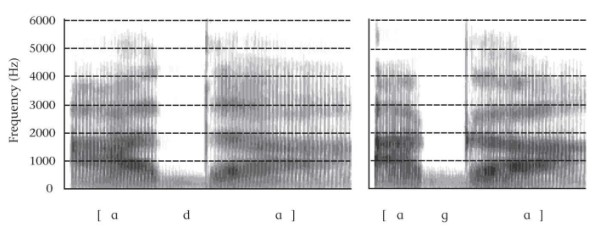
\includegraphics[scale=0.95]{spectrogram_stops_voiced.jpg}
        }
        \only<2>{
          \begin{alertblock}{Aspiration}
            % Definition of aspiration
            % Aspiration
A puff of air following the release of a stop that delays the voicing of the following vowel
, notated with [ʰ]
            \begin{itemize}
              \item In English, this occurs for voiceless stops
            \end{itemize}
          \end{alertblock}
          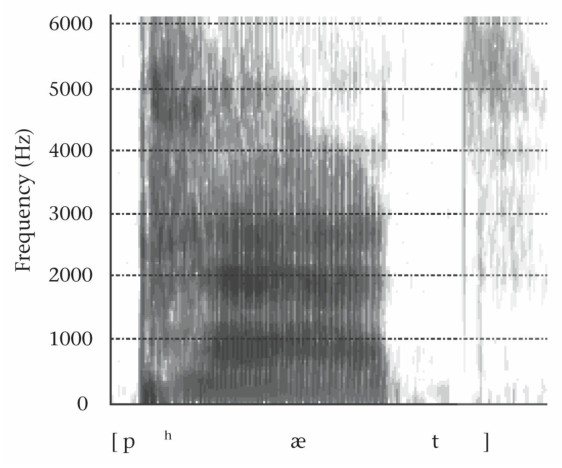
\includegraphics[scale=0.45]{spectrogram_stops_aspirated.jpg}
        }
        \only<3>{
          \begin{block}{Fricatives}
            Appear as high amplitude masses covering large high frequency areas on a spectrogram
            \begin{itemize}
              \item Place of articulation can be determined by how high frequency the areas covered are
            \end{itemize}
          \end{block}
          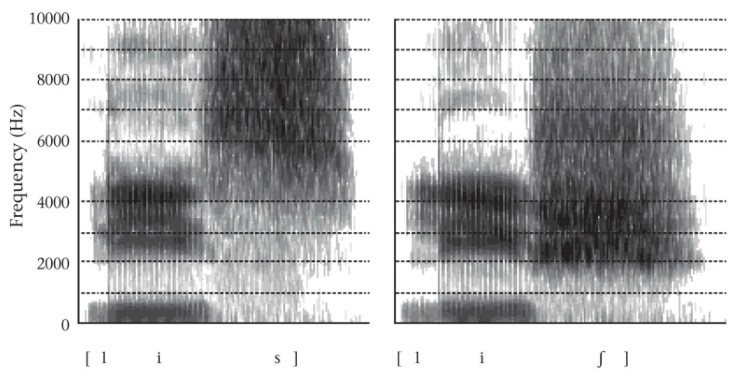
\includegraphics[scale=0.6]{spectrogram_fricatives.jpg}
        }
        \only<4>{
          \begin{block}{Nasals}
            Appear with formants on a spectrogram, like vowels, but the formants shift sharply when transitioning into vowels
            \begin{itemize}
              \item Formants are essentially the same for all nasals
              \item Liquids and glides also have formants
            \end{itemize}
          \end{block}
          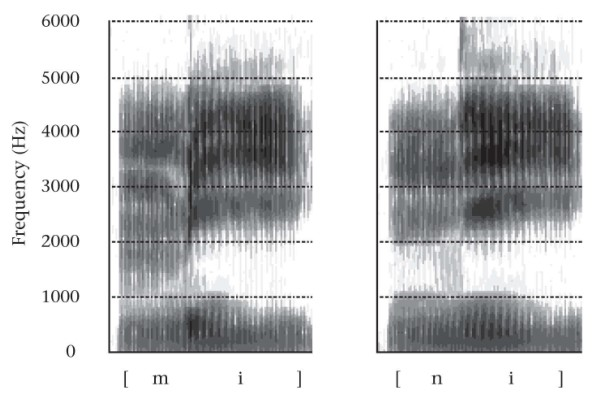
\includegraphics[scale=0.55]{spectrogram_nasals.jpg}
        }
      \end{frame}

    \subsection{\subtwofive}
      \begin{frame}{\subtwofive}
        \begin{block}{Resources}
          % A set of links to useful resources when dealing acoustic phonetics
\begin{itemize}
  \item Use Praat to visualize and measure acoustic information: \url{http://www.fon.hum.uva.nl/praat/}
\end{itemize}

        \end{block}
        \begin{block}{Try these}
          \textcite{dawson_language_2016}, chapter 2 exercises 32 and 33
        \end{block}
      \end{frame}
\end{document}
